\documentclass[letter,12pt]{article}
\usepackage[top=3cm,bottom=2.5cm,left=2.5cm,right=3cm]{geometry}
\usepackage[utf8x]{inputenc}
\usepackage[spanish]{babel}
\usepackage{graphicx}
\usepackage{cite}
\usepackage{hyperref}
\usepackage{lipsum}
\usepackage{tasks}
\usepackage{amsmath}
\newcommand{\eqname}[1]{\tag*{#1}}
\numberwithin{equation}{section}
\usepackage{graphicx,subfigure}
\usepackage{graphicx, amsmath}
\usepackage{chngcntr}
\usepackage{graphicx,wrapfig}
\usepackage{multirow}
\usepackage{rotating}
\usepackage{amssymb}
\usepackage{multicol}
\usepackage{hyphenat}
\usepackage{siunitx}
\usepackage{tikz}

\textwidth=18cm
\textheight=22cm
\topmargin=-2cm
\oddsidemargin=-0.5cm
\decimalpoint
\newcommand\textline[4][t]{%
  \par\smallskip\noindent\parbox[#1]{.333\textwidth}{\raggedright\texttt{+}#2}%
  \parbox[#1]{.333\textwidth}{\centering#3}%
  \parbox[#1]{.333\textwidth}{\raggedleft\texttt{#4}}\par\smallskip%
}
\usepackage{verbatim}
\usepackage{empheq}
 \usepackage[most]{tcolorbox}

\newtcbox{\mymath}[1][]{%
    nobeforeafter, math upper, tcbox raise base,
    enhanced, colframe=blue!30!black,
    colback=blue!30, boxrule=1pt,
    #1}

\DeclareMathOperator{\di}{d\!}
\newcommand*\Eval[3]{\left.#1\right\rvert_{#2}^{#3}}
\usepackage{chngcntr}
\counterwithin{figure}{section}
\usepackage{caption}
\captionsetup[figure]{font=footnotesize, labelfont=footnotesize}
\begin{document}


\thispagestyle{empty}


%%%%%%%%%%%%%%%%%%%%%%%%%%%%%%%%%%%%%%%%%%%%%%%%%%%%%%%%%%
%%                                                                               Capítulo 1                                                                                                     %%       
%%%%%%%%%%%%%%%%%%%%%%%%%%%%%%%%%%%%%%%%%%%%%%%%%%%%%%%%%%



%%%%%%%%%%%%%%%%%%%%%%%%%%%%%%%%%%%%%%%%%%%%%%%%%%%%%
%%%%                                                       Figura: Escudo FCiencias                                                %%%%
%%%%%%%%%%%%%%%%%%%%%%%%%%%%%%%%%%%%%%%%%%%%%%%%%%%%%
%\begin{figure}[h]
%  \begin{center}
%      \includegraphics[scale=0.18,bb=1500 300 1350 400]{Escudo_FCiencias.pdf}
%  \end{center}
%\end{figure}
%%%%%%%%%%%%%%%%%%%%%%%%%%%%%%%%%%%%%%%%%%%%%%%%%%%%%

%%%%%%%%%%%%%%%%%%%%%%%%%%%%%%%%%%%%%%%%%%%%%%%%%%%%%
%%%%                                                         Figura: Escudo UNAM                                                    %%%%
%%%%%%%%%%%%%%%%%%%%%%%%%%%%%%%%%%%%%%%%%%%%%%%%%%%%%
%\begin{figure}[h]
%  \begin{center}
%      \includegraphics[scale=0.14,bb=-2400 10 150 -1100]{Escudo_UNAM.pdf}
%  \end{center}
%\end{figure}
%%%%%%%%%%%%%%%%%%%%%%%%%%%%%%%%%%%%%%%%%%%%%%%%%%%%%
%\vspace{-32mm}
%\centerline{\Large \textbf{ \textsc{Departamento de Física} }}
%\vspace{1mm}
%\centerline{\large \textbf{ \textsc{Facultad de Ciencias} }}
%\vspace{1mm}
%\centerline{\large \textbf{ \textsc{Universidad Nacional Autónoma de México} }}
%\begin{tikzpicture}[yscale=0.5]
%    \draw [line width=0.7mm, blue ] (0,-5) -- (17,-5);
%\end{tikzpicture}
%\vspace{-4mm}
\begin{flushright}
Ciudad Universitaria, a 30 de marzo de 2023
\end{flushright}
\vspace{-1.5mm}
SUBCOMITÉ DE ADMISIÓN DEL POSGRADO EN CIENCIAS FÍSICAS\\
UNIVERSIDAD NACIONAL AUTÓNOMA DE MÉXICO\\
P R E S E N T E \\

\begin{center}
\textbf{PROTOCOLO DE INVESTIGACIÓN PARA EL DOCTORADO}\\
\textbf{del estudiante Jorge Luis Briseño Gómez}
\\
\vspace{0.8 cm}
\textbf{\Large  Transferencia de momento angular de electrones rápidos \\  a nanopartículas}
\end{center}

\section{Antecedentes y justificación del problema}

Desde mediados del siglo pasado, se han propuesto diversos métodos para desarrollar técnicas de manipulación de objetos en la escala micro y nanométrica \cite{ashkin1970acceleration, ashkin1987optical, Ashkin, custance2009atomic, dholakia2011shaping, marago2013optical, romo2020controlled}. Las fuerzas electromagnéticas producidos por haces de luz enfocados, han conducido al desarrollo de las pinzas ópticas, que han demostrado ser de utilidad para atrapar y mover microobjetos, incluidos virus y bacterias, teniendo impacto en el desarrollo tecnológico y médico \cite{ashkin1970acceleration, ashkin1987optical, Ashkin}.  

En 2004, Javier García de Abajo publicó un trabajo donde aborda la posibilidad de manipular nanoobjetos mediante microscopios electrónicos de transmisión (TEMs por sus siglas en inglés) \cite{GarciadeAbajo0}. Posteriormente se observó experimentalmente que los TEM pueden ser usados para inducir movimiento y hacer rotar a nanopartículas (NPs) \cite{Batson01, zheng2012electron}, lo cual ha motivado al desarrollo de una nueva técnica de manipulación llamada <<pinzas electrónicas>> \cite{Batson, oleshko2005electron, Oleshko}, en analogía con las pinzas ópticas. En diversos estudios experimentales sobre pinzas electrónicas, se ha observado que la transferencia de momento angular y lineal del haz de electrones a la NP, depende tanto de la velocidad con la que viaja el haz de electrones así como del parámetro de impacto, que es la distancia efectiva entre la trayectoria del haz de electrones y el centro de la NP \cite{OLESHKO2013203, Oleshko, Batson, Batson01, zheng2012electron, xu2010transmission}.  Se ha mostrado que al modificar el parámetro de impacto, la interacción entre el haz de electrones y la NP puede ser atractiva o repulsiva, y también se ha reportado que es posible modificar la dirección del giro inducido sobre la NP \cite{OLESHKO2013203, Batson, Oleshko}. 

El STEM forma imágenes mediante haces enfocados de electrones, barriendo con él muestras, utilizando los electrones esparcidos por ellas \cite{Batson}. En la Fig. \ref{fig: Batson STEM} se observa un par de NPs de oro (en color amarillo): una grande, a la izquierda de la figura, y una pequeña, dentro de la región con contorno blanco a la derecha. La NP de oro pequeña está siendo escaneada por el haz de un STEM, barriendo la región delimitada por el contorno blanco. El haz de electrones permanece detenido 20\% del tiempo de barrido al inicio de cada una de las líneas a escanear, produciendo una corriente neta de electrones que viajan fuera de la NP, ilustrada como una región sombreada en azul en la Fig. \ref{fig: Batson STEM}. Por lo anterior, se puede afirmar que, aunque el haz barre toda la muestra que se observa en el STEM, hay un parámetro de impacto efectivo respecto a la superficie de la NP.

\begin{figure}[h!]
\centering
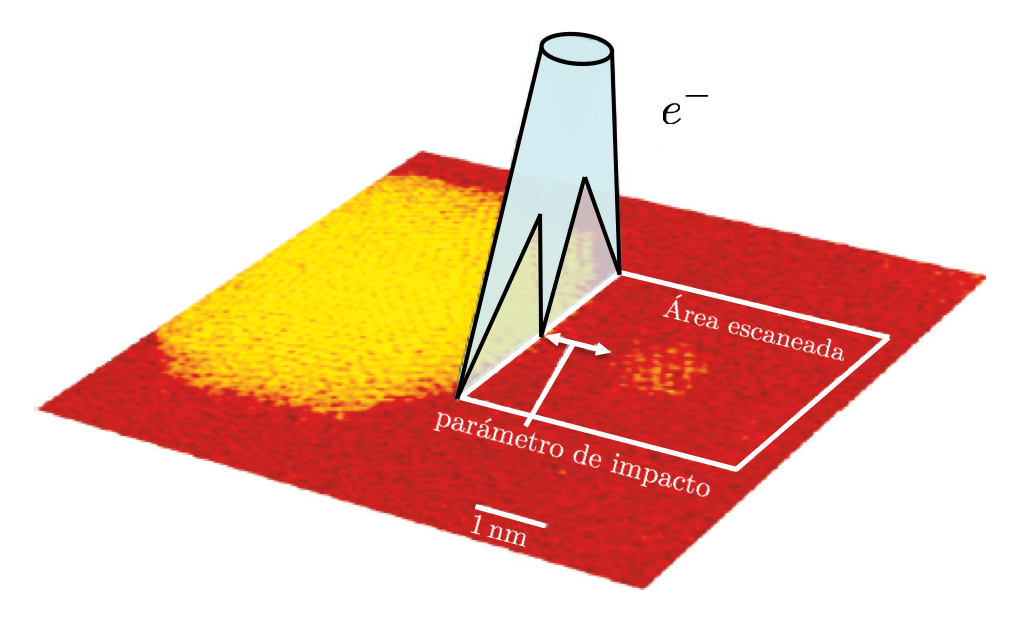
\includegraphics[width=0.6\linewidth]{17-imagenes/1-Intro/STEM}
\caption{\label{fig: Batson STEM} Esquema de la interacción dentro de un STEM, entre un haz de electrones con un par de nanopartículas de oro, reproducido y adaptado de la Ref \cite{Batson}.} 
\end{figure}

En la Fig. \ref{fig: Batson momentum transfer} se muestran algunos de los resultados reportados en la Ref. \cite{Batson}. En la Fig. \ref{fig: Batson momentum transfer} se observan seis imágenes de STEM de una NP de oro de $1.5$ nm en presencia de otra de $5$ nm, a distintos tiempos. En todas las imágenes de la Fig. \ref{fig: Batson momentum transfer}, el parámetro de impacto efectivo se encuentra a la izquierda de la NP (cerca del borde de la imagen). Las tres imágenes superiores de la Fig. \ref{fig: Batson momentum transfer}, tomadas con un parámetro de impacto efectivo de $4.5$ nm, muestran una interacción atractiva entre el haz y la NP, pues se puede apreciar que la NP se acerca al borde izquierdo de las imágenes, atravesando la línea punteada color blanco colocada como una ayuda al ojo. Por el contrario, en las imágenes inferiores de la Fig. \ref{fig: Batson momentum transfer}, cuyo  parámetro de impacto efectivo es de $1$ nm,  se observa que la NP se aleja del haz, atravesando la línea punteada blanca en dirección opuesta y acercándose al borde derecho de la imagen, indicando una interacción repulsiva. Además, puede apreciarse en la Fig. \ref{fig: Batson momentum transfer} es el giro de las nanopartículas inducido por el haz de electrones a las NPs. Por ejemplo, utilizando las líneas guía que se han trazado en las facetas de la NP más grande de la Fig. \ref{fig: Batson momentum transfer} y que forman un polígono, puede apreciarce que en las tres imágenes superiores, dicha NP gira en sentido horario mientras que en las inferiores, al cambiar el parámetro de impacto, gira en sentido antihorario.

\begin{figure}[h!]
\centering
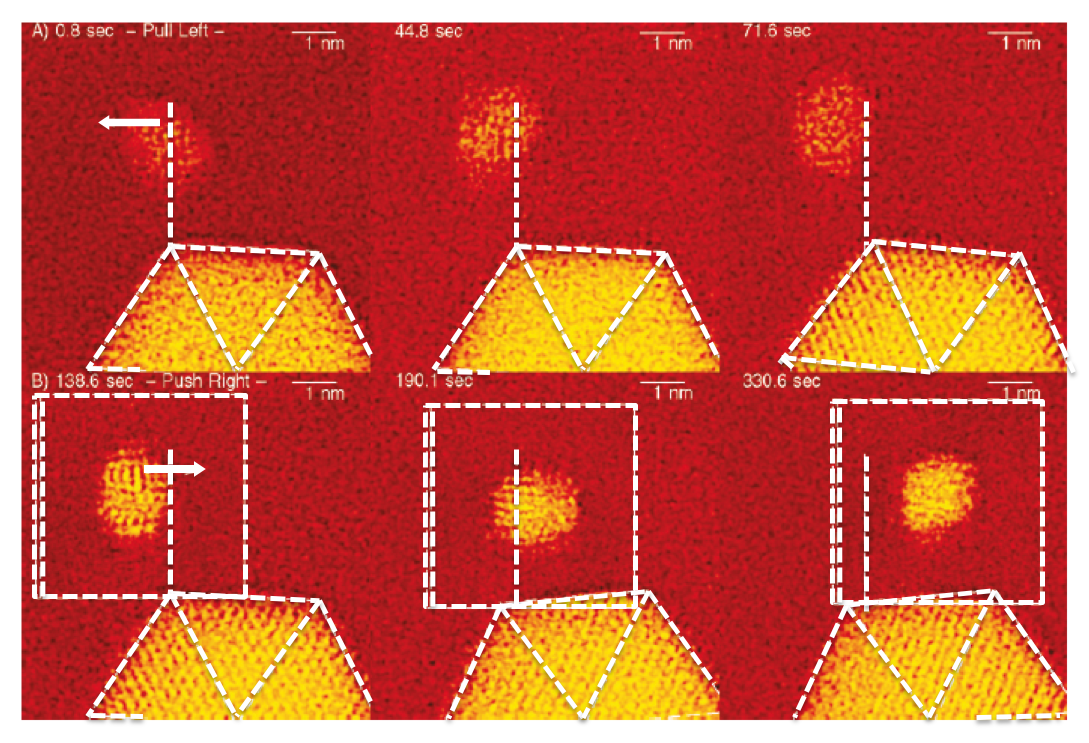
\includegraphics[width=0.6\linewidth]{17-imagenes/1-Intro/Batson}
\caption{\label{fig: Batson momentum transfer} Resultados reproducidos y adaptados de la Ref. \cite{Batson}, donde se observa transferencia de momento angular y lineal de un haz de electrones STEM a nanopartículas de oro, suspendidas en un sustrato de carbono.} 
\end{figure}

Para el desarrollo de la técnica de pinzas electrónicas, es necesario un entendimiento teórico del problema. La interacción de haces de electrones con nanopartículas esféricas ha sido abordado desde la perspectiva de la electrodinámica clásica \cite{GarciadeAbajo0, PRBCoronado, Lagos2, Batson2, xu2010transmission}, mediante la solución de las ecuaciones de Maxwell en el espacio de frecuencias. Los trabajos citados anteriormente se han centrado en el cálculo de transferencia de momento lineal, mediante el cálculo de una integral de superficie cerrada alrededor de la NP y una integral en el espacio de frecuencias. En estos trabajos, los campos electromagnéticos producidos por el electrón y la NP, se pueden expresar en una base esférica en términos de una expansión multipolar, lo que permite separar la contribución eléctrica y magnética de la interacción, así como también separar la contribución de cada orden multipolar. A pesar de que estos trabajos han logrado reproducir el comportamiento atractivo y repulsivo de la interacción, estudios recientes han mostrado que dichos trabajos obtuvieron resultados no físicos al modelar la respuesta electromagnética de la NP mediante funciones dieléctricas no causales \cite{castrejon2021effects, castrejon2021phdthesis}. En los trabajos citados anteriormente, se muestra que no aparece la interacción repulsiva reportada experimentalmente, si se elimina el comportamiento no causal de las funciones dieléctricas. La Ref. \cite{castrejon2021phdthesis} resuelve de forma semi-analítica las integrales en el espacio de frecuencia, que previamente se resolvían de forma numérica en las Refs. \cite{GarciadeAbajo0, PRBCoronado, Lagos2, Batson2, xu2010transmission}. Lo anterior permite conocer de manera exacta la contribución en el espacio de frecuencias de cada multipolo a la transferencia de momento lineal, logrando así calcular la transferencia de momento lineal, de electrones rápidos a NPs grandes (de hasta $a=50$ nm de radio). 

Se ha mostrado que, tanto para el caso lineal como el angular, existen términos del tensor de esfuerzos de Maxwell correspondientes a los campos del electrón, que no contribuyen a la transferencia de momento total. Por otra parte, se ha mostrado que el término de interacción en el tensor de esfuerzos, que incluye tanto al campo del electrón como al campo esparcido por la NP, es el que más contribuye a la transferencia de momento; y que el término que incluye únicamente a los campos esparcidos por la NP, a pesar de ser menor, no se anula. Lo anterior da pie a una transferencia de momento total debida a la reacción de radiación \cite{castellanos2021phdthesis, castrejon2021phdthesis}. También se ha mostrado que un ajuste no adecuado a datos experimentales, conlleva a predecir resultados no físicos. Como experimentalmente se mide la función dieléctrica en un rango finito de frecuencias, se debe extrapolar e interpolar para realizar la integral del tensor de esfuerzos de Maxwell en todo el espacio de frecuencias. Este proceso puede dar como resultado una función dieléctrica no causal, que no satisface las relaciones de Kramers-Kronig, y se ha demostrado que puede predecir resultados repulsivos que no son físicos al provenir de una respuesta no causal \cite{castrejon2021phdthesis}. 

El cálculo de la transferencia de momento angular (TMA) solo había sido discutido brevemente en trabajos posteriores a 2021 (ver por ejemplo la Ref. \cite{GarciadeAbajo-1}). A pesar de lo anterior, un estudio detallado de la dinámica angular es imprescindible para el desarrollo de la técnica de pinzas electrónicas. Recientemente se han publicado estudios de la TMA de electrones rápidos a NPs pequeñas, de hasta $a=5$ nm de radio \cite{castellanos2021phdthesis, castellanos2021angular,castellanos2023theory}, donde se usan dos métodos para calcular la TMA: \textbf{(1)} modelando la respuesta electromagnética de la NP como un dipolo puntual y \textbf{(2)} resolviendo numéricamente las integrales de superficie y en el espacio de frecuencias. Resolver numéricamente la integral de superficie para la TMA puede representar un problema en cuanto a los tiempos de cómputo, al calcular la TMA para NPs grandes. Ambas metodologías, mencionadas con anterioridad, solo permiten el cálculo de la TMA para NPs pequeñas. Una comparativa entre el avance logrado entre el caso lineal con el angular, sugiere que es necesario encontrar soluciones semi-analíticas en el espacio de frecuencias para disminuir el tiempo de cómputo en el cálculo de la TMA, y así poder estudiar la dinámica angular en la interacción de electrones rápidos con NPs grandes de hasta $a=50$ nm de radio. 

Los haces electrónicos en un STEM pueden alcanzar los $400$ keV de energía cinética, con una corriente eléctrica del orden de pA, lo que equivale a un pulso de electrones rápidos viajando a velocidad constande alcanzando velocidades de hasta $v=0.83 c$ (donde $c$ es la velocidad de la luz). De lo anterior, se tiene que el tiempo de emisión de cada electrón es de $10^{-8}$ s. Como la vida media de las excitaciones dentro de un metal es de $\sim 10^{-14}$ \cite{quijada2010lifetime}, se puede asumir que la NP interactúa con un electrón a la vez \cite{de1999relativistic, GarciadeAbajo-1, deabajo2021optical}. Además,  los haces de electrones en estudios de STEM se desvian a ángulos del orden de miliradianes \cite{deabajo2021optical, Rivacoba1, krehl2018spectral}, por lo que se puede considerar que se mueven en línea recta siempre y cuando no incidan sobre las muestras. 

\begin{figure}[ht!]
\centering
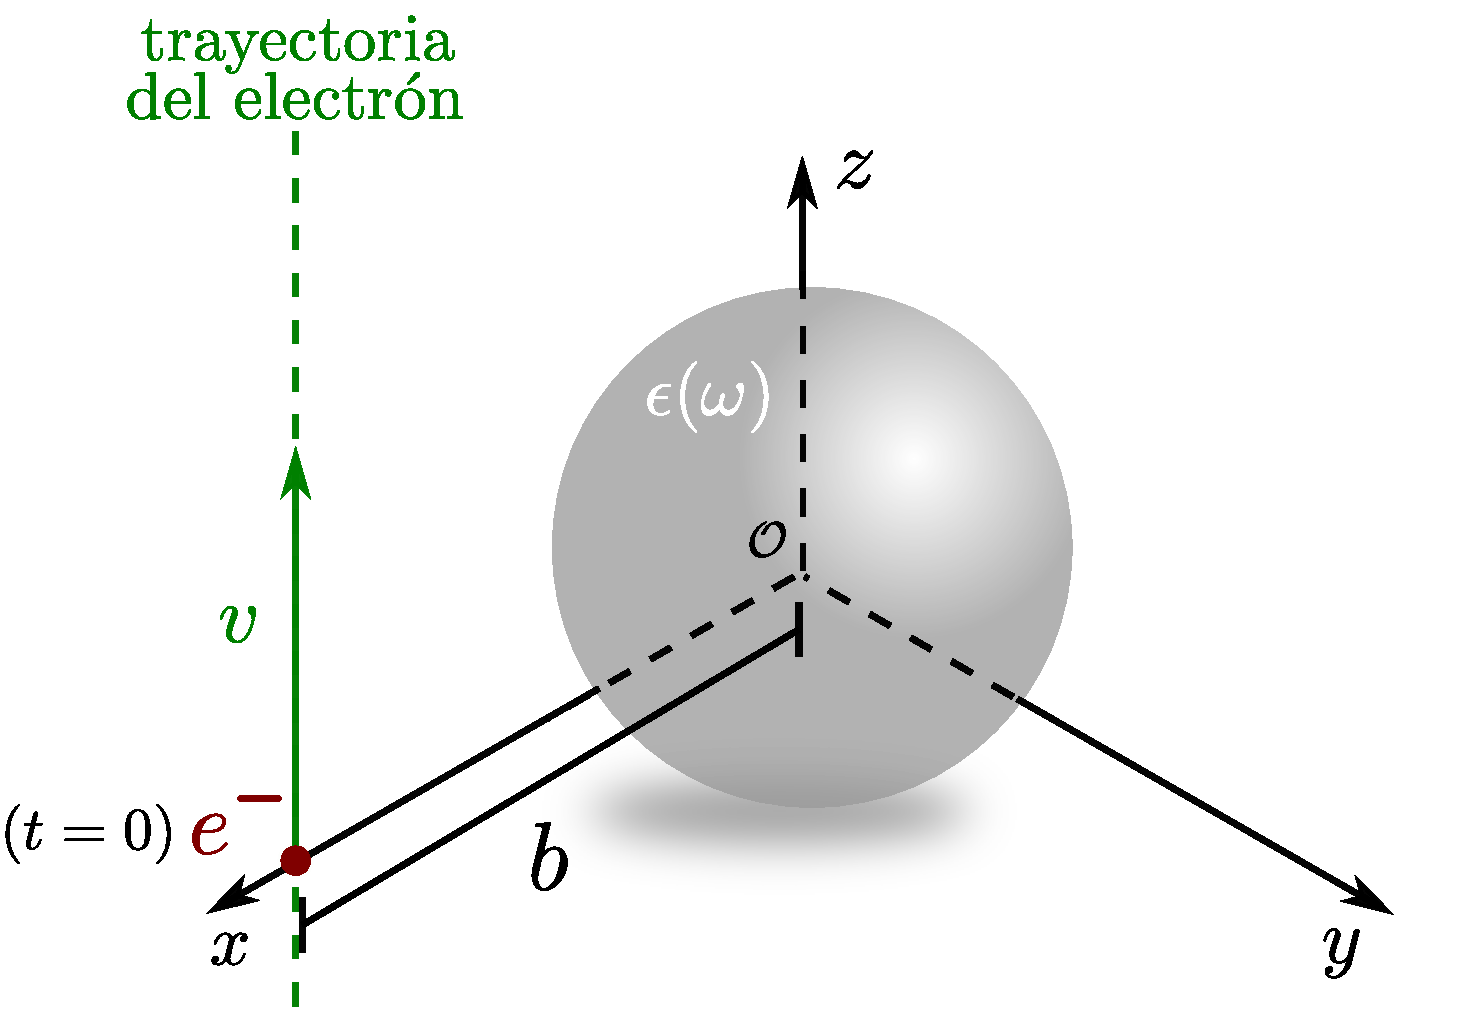
\includegraphics[width=0.5\linewidth]{17-imagenes/1-Intro/system.pdf} 
\caption{Nanopartícula de radio $a$, centrada en el origen de coordenadas, modelada mediante una función dieléctrica $\epsilon(\omega)$ en vacío. La trayectoria del electrón (punto marrón), con parámetro de impacto $b$ y viajando a velocidad constante $v$, se muestra como una línea punteada de color verde. }
\end{figure}

\section{Desarrollo}

Aunque actualmente se cuenta con una metodología para el cálculo de la transferencia de momento angular, debido a limitaciones de eficiencia no ha sido posible calcularla para NPs mayores a $5$ nm de radio. Las integrales del tensor de esfuerzos de Maxwell sólo han sido resueltas numéricamente para el caso angular, volviendo el cálculo cada vez más tardado conforme crece el número de multipolos a considerar en NPs grandes \cite{castellanos2021phdthesis}. Mediante una solución semianalítica de la transferencia de momento angular, se puede reducir el tiempo de cómputo de la transferencia de momento angular para NPs grandes, lo cual no había sido explorado con anterioridad.

Durante mis estudios de maestría calculé de forma semianalítica la transferencia de momento angular del electrón hacia la NP, obteniendo expresiones generales para NPs caracterizadas por una función dieléctrica local $\epsilon (\omega)$. Durante mi primer año de doctorado, la propuesta de trabajo que se plantea es utilizar el formalismo desarrollado durante la tesis de maestría para desarrollar un programa en lenguaje C que calcule la transferencia de momento angular, y comparar con resultados ya publicados para NPs pequeñas \cite{castellanos2021angular}, y posteriormente calcular la transferencia de momento angular para NPs grandes (de hasta $50$ nm de radio). Los objetivos generales para el trabajo de doctorado son el calcular la transferencia de momento angular de electrones rápidos a NPs en un amplio rango de tamaños y distintos tipos de materiales (dieléctricos y plasmónicos), en función de los parámetros relevantes del problema (parámetro de impacto y velocidad de los electrones). Se propone explorar el comportamiento de la interacción usando funciones dieléctricas espacialmente locales y no locales, porque experimentalmente se observa la interacción atractiva y no se ha podido explicar con los modelos publicados hasta el momento.

\section{Objetivos}



\bibliographystyle{unsrt} 
\bibliography{references-links-arc}

\vfill


\qquad \, \,  {A T E N T A M E N T E}  \, \, \, \, \, \, \,   \, \, \, \, \, \, \, \, \, \, \,   \, \, \, \, \, \, \, \, \, \, \,  \textbf{Vo. Bo.}

\vspace{3mm}

\includegraphics[scale=.25]{signature}\qquad \\
\rule{0.4\textwidth}{0.4mm}  \qquad  \,   \rule{0.47\textwidth}{0.4mm} 

\qquad {\textbf{Jorge Luis Briseño Gómez}} \qquad \qquad \,   \, \,   \, \,  \textbf{Dr. Alejandro Reyes Coronado}

\quad \, Estudiante de la carrera de Física \qquad \,  \, \,  \, \,   Profesor Titular ``B” de Tiempo Completo

\qquad \qquad No. Cuenta 414010248 \qquad \qquad \, \, \, \,  Depto. de Física, Facultad de Ciencias, UNAM

\qquad \, \, \, Tel. +52 55 23 18 36 91 \qquad  \, \, \, \, \, \, \, \, \,  Ciudad Universitaria, Av. Universidad 3000

e-mail: jorgeluisbrisenio@ciencias.unam.mx \qquad     \, \, \, \,   \, \, \, \, Ciudad de México, México

\qquad \, \, \, \, \, \, \,   \, \, \, \, \, \, \, \, \, \,   \, \, \, \, \, \, \, \, \, \, \,   \, \, \, \, \, \, \, \, \, \, \,  \, \, \, \, \, \, \, \,    Tel.: (52 55) 5622 4968

\qquad \, \, \, \, \, \, \,   \, \, \, \, \, \, \, \, \, \, \,   \, \, \, \, \, \, \, \, \, \, \,   \, \, \, \, \, \, \, \, \, \, \,   \, \,  e-mail: coronado@ciencias.unam.mx
\end{document}